\section{绘图命令}
SAC提供了许多与绘图有关的命令,包括控制图像外观的参数控制类命令以及执行绘图功能
的操作执行类命令。这一节将介绍常用的几个操作执行类命令。

\subsection{plot}
plot命令会绘制内存块中的所有波形数据,但每次只显示一个波形,然后等待用户输入
再决定是否显示下一个波形。该命令的具体用法在第~\ref{sec:display}节已经详细介绍。

\subsection{plot1}
plot1命令会绘制内存块中的所有波形数据,在一个窗口中一次显示多个波形,
这些波形共用一个X轴(时间轴),但拥有单独的Y轴。

\begin{SACCode}
SAC> dg sub local cdv.[enz]
cdv.e cdv.n cdv.z
SAC> p1
\end{SACCode}

执行plot1命令后,焦点位于图形窗口,显示如图~\ref{fig:plot1}。
\begin{figure}[H]
\centering
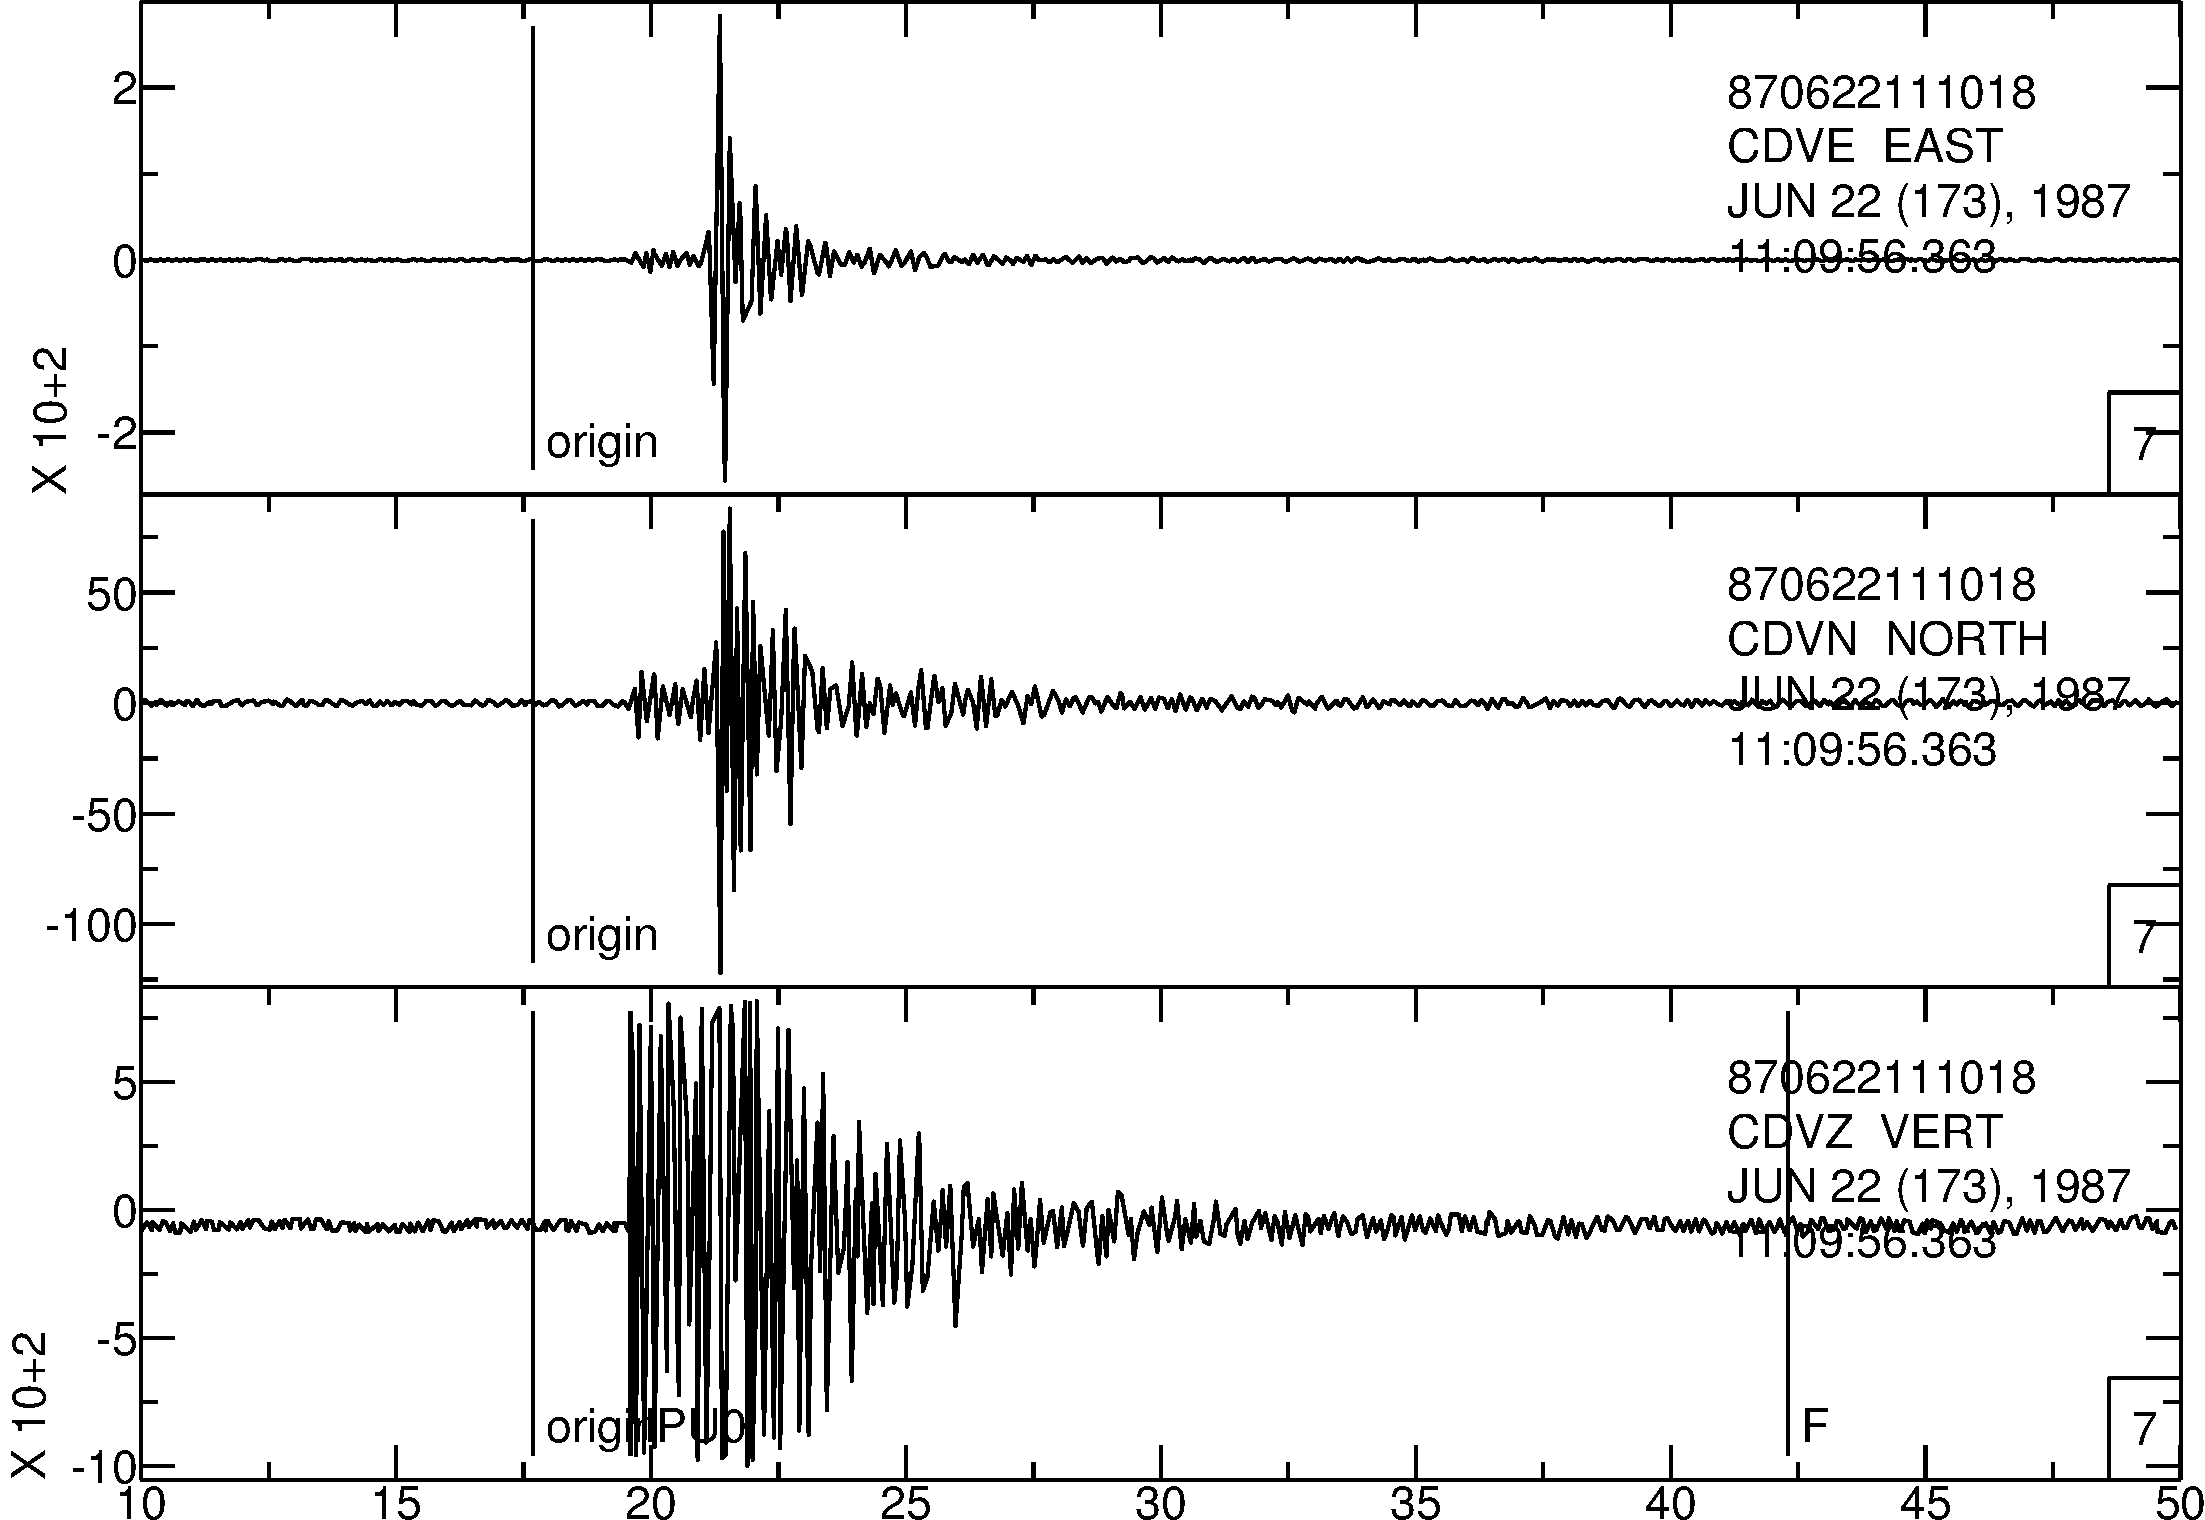
\includegraphics[width=0.85\textwidth]{plot1}
\caption{plot1绘图效果}
\label{fig:plot1}
\end{figure}

当一次性读入多个波形数据时,若直接使用plot1绘图,会一次性显示全部波形,导致
窗口内波形太密,反而什么都看不清。plot1提供了``\verb+perplot n+''选项以
指定窗口内一次最多显示多少个波形,余下的波形则处于等待状态。在查看波形的时候,
经常需要将每个台站的三分量波形记录放在一起看,此时设置选项
~\verb+perplot+~的参数值为~\verb+3+即可。
\begin{SACCode}
SAC> dg sub local cdv.[enz] cvl.[enz] cvy.[enz]  // 生成9个地震波形
cdv.e cdv.n cdv.z cvl.e cvl.n cvl.z cvy.e cvy.n cvy.z
SAC> p1 p 3         // p是选项perplot的简写,3代表每次显示3个波形
Waiting
Waiting
SAC>
\end{SACCode}

默认情况下,所有的波形数据会按照绝对时间(~\verb+absolute+)对齐,若波形数据
具有不同的开始时间,则波形数据之间会出现相对错动;也可以使所有的波形数据相对于
(~\verb+relative+~)各自的开始时间绘图,此时X轴的起始坐标为0。

\subsection{plot2}
plot2会一次性将内存块中的所有波形绘制在一个窗口内,所有的波形共用X轴,因而绘图
时也可以使用绝对模式或相对模式。与plot1不同的是,所有的波形还同时共用Y轴,因而
波形会相互覆盖。

plot2适合绘制多个波形的对比图,常用于数据处理前后波形对比或真实波形与合成波形间的对比。
\begin{SACCode}
SAC> fg seis                     // 生成数据
SAC> rmean; rtrend; taper        // 预处理
SAC> w seis.0                    // 写入滤波前文件
SAC> bp c 0.05 10 n 4 p 2        // 滤波
SAC> w seis.1                    // 写入滤波后文件
SAC> r ./seis.[01]               // 读入两个文件
./seis.0 ...seis.1
SAC> color red inc list red blue // 对两个数据分别设置红色和蓝色
SAC> p2                          // 绘图
\end{SACCode}
图~\ref{fig:plot2}~中红线为滤波前波形,蓝线为滤波后波形,二者共用X轴和Y轴,
从这样的波形对比图中,可以很明显得看到滤波对于波形的影响。

\begin{figure}[H]
\centering
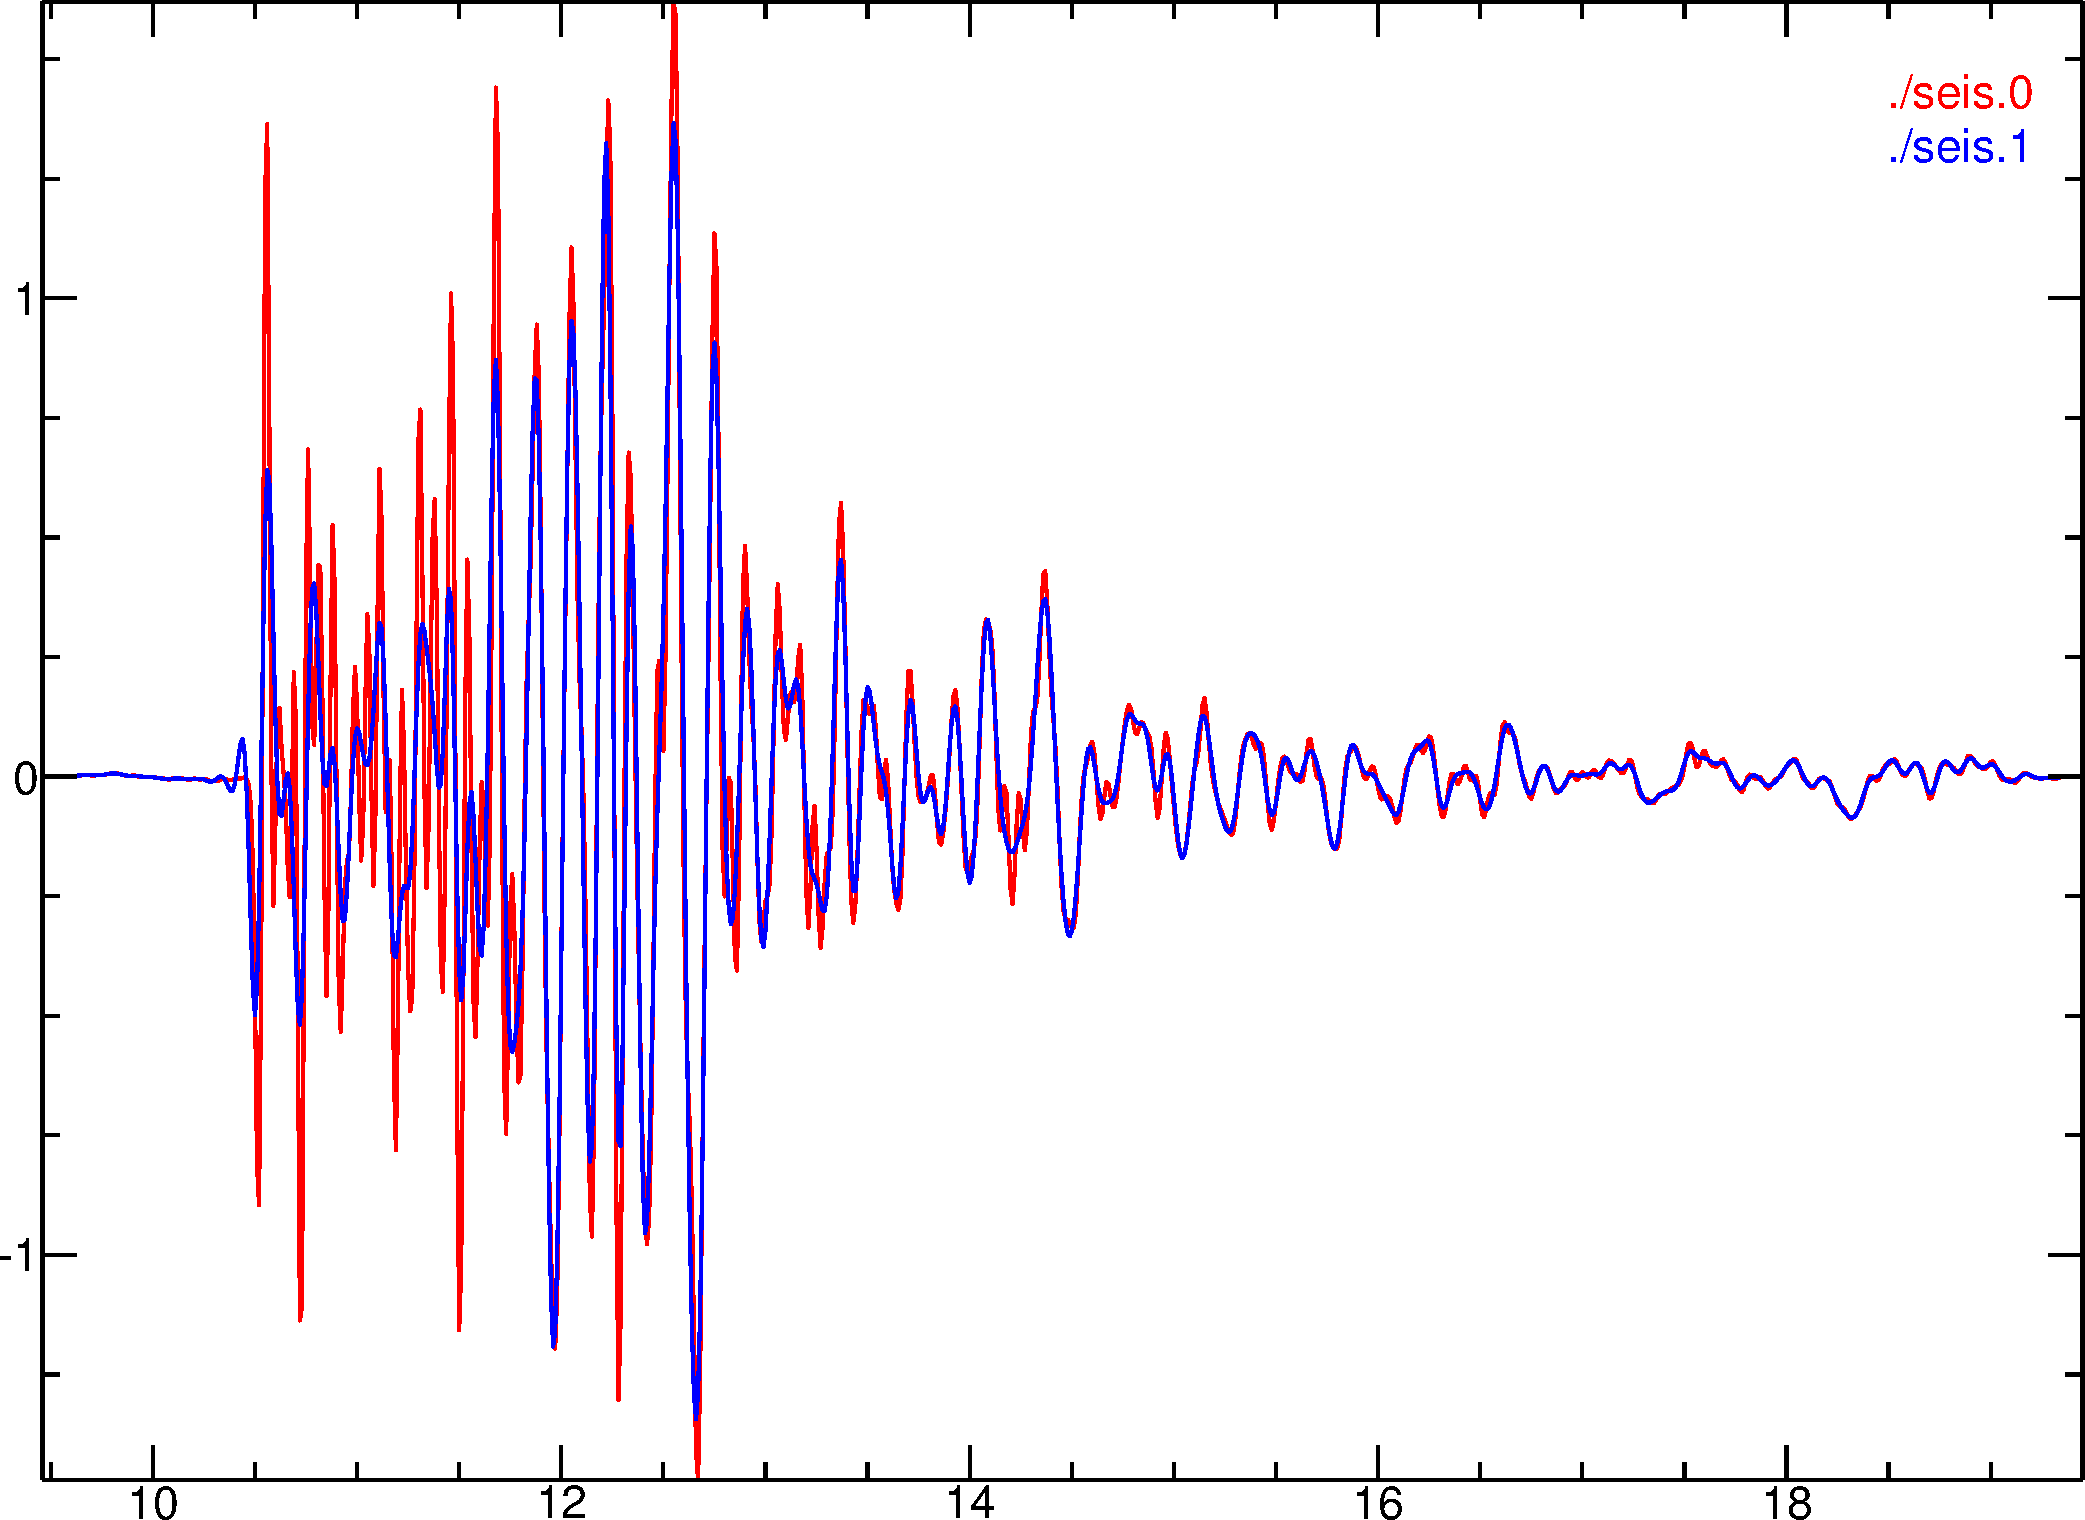
\includegraphics[width=0.85\textwidth]{plot2}
\caption[plot2绘图效果]{plot2绘图效果。红色为滤波前波形,蓝色为滤波后波形。}
\label{fig:plot2}
\end{figure}

\subsection{plotpk}
plotpk是SAC中最常用的命令之一。其可以在窗口中显示指定个数的波形,所有波形共用X轴,
但拥有单独的Y轴。该命令主要用于震相拾取,在``~\nameref{sec:phase-picking}~''一节
有详细介绍。

\subsection{plotpm}
plotpm可以利用成对的波形数据,提取出任一时间段内两个波形数据的振幅信息,绘制在
``振幅-振幅''图中。若一对波形数据恰好是同一台站两个互相垂直的分量,
则``振幅-振幅''图即为``质点运动图''。从``质点运动图''中,可以提取出震相的一些重要信息。

下面的例子利用垂直和径向分量的波形数据绘制Rayleigh面波的质点运动轨迹:
\begin{SACCode}
SAC> dg sub tele nykl.z             // Z分量
SAC> w nykl.z
SAC> dg sub tele nykl.e nykl.n      // E、N分量
SAC> rotate to gcp                  // 旋转至大圆路径
SAC> w nykl.r nykl.t                // R、T分量
SAC> r nykl.z nykl.r                // 读入Z和R分量
SAC> xlabel 'Radial component'
SAC> ylabel 'Vertical component'
SAC> title 'Particle-motion plot for partial Rayleigh wave'
SAC> xlim 1300 1340                 // 仅绘制Rayleigh面波的部分时间窗
SAC> ppm                            // 绘制质点运动图
\end{SACCode}

鉴于SAC的ppm命令绘图的效果很糟糕,就不再贴效果图了,读者可以根据上面的命令自行绘制。

\subsection{plotsp}
plotsp命令用于绘制不同格式的谱文件,可以绘制``振幅+相位''或者``实部+虚部'',
同时可以任意指定X、Y轴为线性轴或对数轴。

下面的命令对波形数据进行FFT得到谱文件,并使用plotsp命令绘制其振幅谱:
\begin{SACCode}
SAC> fg seis
SAC> fft
SAC> psp am loglog
\end{SACCode}

\begin{figure}[H]
\centering
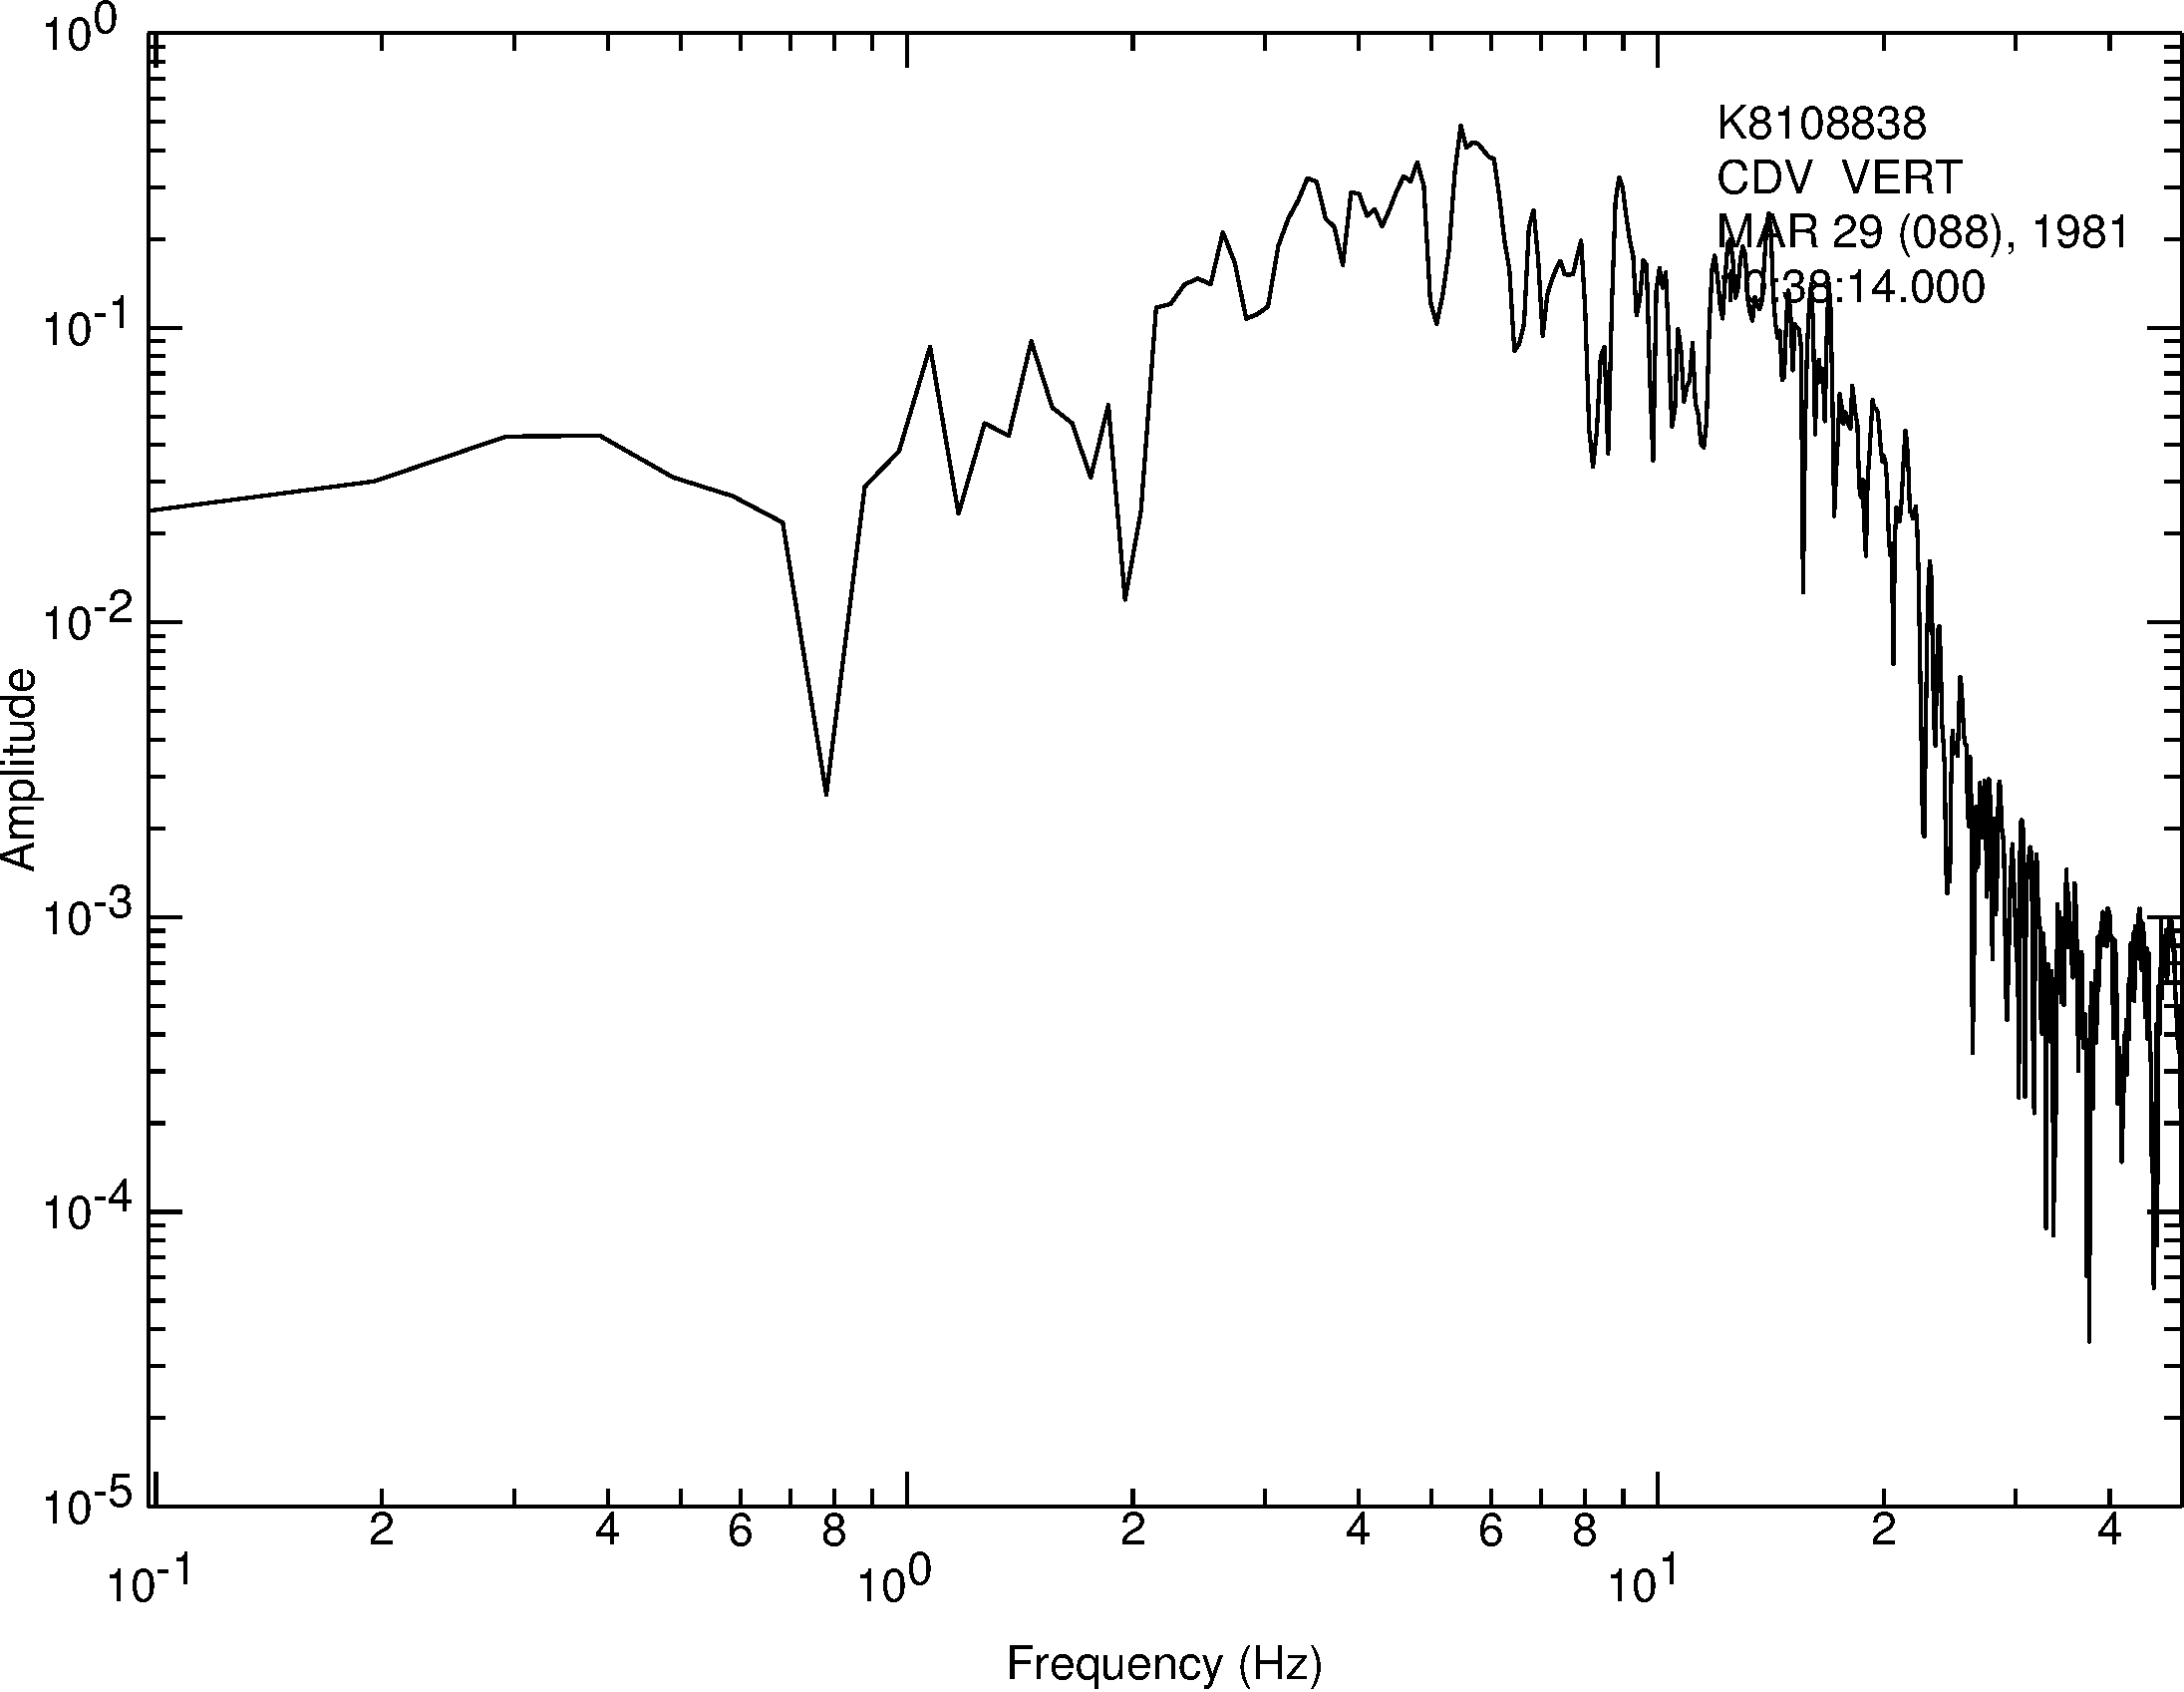
\includegraphics[width=0.95\textwidth]{plotsp}
\caption{plotsp绘制振幅谱}
\label{fig:plotsp}
\end{figure}
